% This is LLNCS.DEM the demonstration file of
% the LaTeX macro package from Springer-Verlag
% for Lecture Notes in Computer Science,
% version 2.3 for LaTeX2e
%
\documentclass{llncs}
%
\usepackage{ngerman}
\usepackage[T1]{fontenc}
\usepackage[utf8]{inputenc}
\usepackage{makeidx}  % allows for indexgeneration
\usepackage{multirow}
\usepackage{rotating}
\usepackage{verbatim}
\usepackage{graphicx}
\usepackage{amssymb}   % AMS-Sonderzeichen
\usepackage{tabularx}  % Für tabularx und newcolumntype
% \usepackage[paper=a4paper,left=30mm,right=30mm,top=30mm,bottom=30mm]{geometry}
\usepackage{color}
\usepackage{ragged2e}
\usepackage{ifpdf}
% \usepackage{titlesec}
\usepackage{xcolor}    % Lieber xcolor als color. Dann klappt auch das listings gut mit den Farben
\usepackage{listings}
\usepackage{upquote}   % Verändert die Ausgabe der einfachen Anführungszeichen innerhalb von verbatim
\usepackage{eurosym}   % Euro-Zeichen: \euro
\usepackage{lastpage}  % \pageref{LastPage} um die Anzahl der Seiten zu erhalten
% hiermit kann man auch umlaute copy-pasten
\usepackage{lmodern}
\selectlanguage{english}
\usepackage{fancyhdr}
\pagestyle{fancy}
%

\ifpdf
\pdfinfo{
   /Author (Wladymir Alexander Brborich Herrera)
   /Author (Vishwaben Pareshbhai Kakadiya)
   /Author (Hellyben Bhaveshkumar Shah)
   /Author (Priyanka Dilipbhai Vadiwala)
   /Author (Heer Rakeshkumar Vankawala)
   /Title  (LowTech GMmBH Techincal Transformation Milestone 1)
   /Subject (Cloud Computing)
   /Keywords (Cloud Computing, Technical Transformation, Migration)
}
\fi

\setlength{\parindent}{0pt}    % Erste Zeile eines Absatzes nicht einrücken
\parskip2ex                    % Absatzabstand
\setlength{\itemsep}{0ex plus0.2ex}
\sloppy                        % Auf jeden Fall die Seitenränder einhalten.

\newcommand{\what}{LowTech GMmBH Techincal Transformation Milestone 1}
\newcommand{\who}{Group 23}
\newcommand{\when}{WiSe 2024-2025}

\renewcommand{\headrulewidth}{0.4pt}
\renewcommand{\footrulewidth}{0.4pt}
\lhead[\when]{\who}
\rhead[\who]{\when}
\chead[]{}
\lfoot[Page \thepage\ of \pageref{LastPage}]{\what}
\rfoot[\what]{Page \thepage\ of \pageref{LastPage}}
\cfoot[]{}
\pagestyle{fancy}


% Hurenkinder und Schusterjungen komplett verbieten.
\clubpenalty = 10000 
\widowpenalty = 10000 
\displaywidowpenalty = 10000
% Diese Begriffe bezeichnen den Makel beim Textsatz, wenn eine Seite mit der ersten Zeile eines Absatzes endet (so genannter Schusterjunge) oder eine neue Seite mit der letzten Zeile eines Absatzes beginnt (so genanntes Hurenkind).


% Wir definieren ein paar Farben
\definecolor{Brown}{cmyk}{0,0.81,1,0.60}
\definecolor{OliveGreen}{cmyk}{0.64,0,0.95,0.40}
\definecolor{CadetBlue}{cmyk}{0.62,0.57,0.23,0}
\definecolor{lightlightgray}{gray}{0.9}
\definecolor{FrankfurtBlue}{HTML}{3333b2}

% Hier fängt das Dokument an!
\begin{document}

%
% \frontmatter          % for the preliminaries
%
% \tableofcontents
%
\mainmatter              % start of the contributions
%
\title{\what}
%
\author{
  Wladymir Alexander Brborich Herrera\\
  \texttt{wladymir.brborich-herrera@stud.fra-uas.de}
  \and\\ 
  Vishwaben Pareshbhai Kakadiya\\
  \texttt{}
  \and\\
  Hellyben Bhaveshkumar Shah\\
  \texttt{}
  \and\\
  Priyanka Dilipbhai Vadiwala\\
  \texttt{}
  \and\\
  Heer Rakeshkumar Vankawala\\
  \texttt{}
}
%
\institute{
  Frankfurt University of Applied Sciences\\
  (1971-2014: Fachhochschule Frankfurt am Main)\\
  Nibelungenplatz 1\\
  D-60318 Frankfurt am Main\\
}

\maketitle              % typeset the title of the contribution

\begin{abstract}
  LowTech GMmBH is a wooden furniture retailer that went public with an online store several years ago. To do so they implemented an on-premise solution. Which not only drives the online store, but all the auxiliary applications i.e. warehouse, customer service, finance and HR software. As demand increases, they are looking to modernize the current infrastructure using a private cloud. This document provides an in depth analysis of of the current infrastructure, including energy consumption metrics, the proposed roadmap and technologies to perform the technical transformation, and finally, a list of potential benefits of the approach, including a simple cost analysis.
  
\end{abstract}

This is where the introduction (the prologue or foreword) comes in. The introduction should also be short and concise. The reader should be prepared for the text that follows. Of course, the introduction should also be formulated in an interesting way.

\section{Overview of the problem}

LowTech GmbH has seven departments with all of their infrastructure hosted on premise. The original partner in charge of the infrastructure has gone out of business


\section{Objectives of the technological transformation}

The main high level objective is to migrate the current infrastructure into a private-cloud context, meaning that we are going to rent server space and manage only the software components of the technology stack. The hardware maintenance and provisioning will be handled by a third party. We expect to have an improvement in performance just by the fact that we will be using newer/faster technologies, nevertheless, we expect at least parity with the current implementation. 


\section{Assessment of the current infrastructure}

\subsection{Current traffic and usage}

\subsection{Approximate energy consumption}

\subsection{Scalability, availability and security analysis}




\section{Client Requirements}

\begin{itemize}
  \item Make the infrastructure more scalable, available and secure
  \item Modernize the technology, runtime and operation modality
  \item Perform the migration with a maximum downtime of 4 hours
  \item Cost reduction
  \item Maintenance reduction
  \item High availability of 99.5\%
\end{itemize}

\section{Assessment of potential technological components}

\subsection{Hardware}

\begin{itemize}
  \item Provisioning modern hardware locally
  \item Renting server space
\end{itemize}

\subsection{Virtualization technologies}


\subsection{Application components}

\subsection{Platforms}

\subsection{Security components}


\section{Migration to a private-cloud context}

To perform a successful migration to a private cloud context we have analyzed the baseline performance of the current system, as well as the technologies used. Based on the client requirements, we have selected technologies and established a roadmap to perform this task.   

\subsection{Selected technologies}

\begin{itemize}
  \item Virtualization engine
  \item Storage arrangement
  \item 
\end{itemize}

\newpage

\subsection{Architecture}

\begin{figure}[htbp]
  \begin{center}
    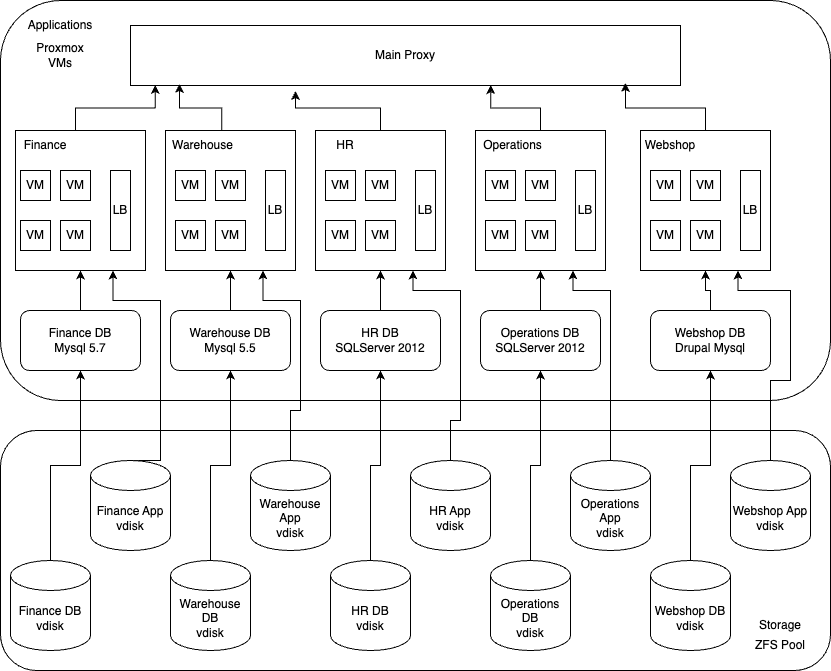
\includegraphics[width=12cm]{diagrams/architecture.drawio.png}
    \caption{High Level Architecture~\ref{High_Level_Architecture}}
    \label{High_Level_Architecture} % A unique label.
  \end{center}
\end{figure}

\section{Roadmap}

The technological transformation roadmap is divided in four phases:
\begin{itemize}
  \item Assessment
  \item Design
  \item Execution
  \item Optimization
\end{itemize}

\subsection{Assessment}
This is one of the most critical steps, given that we need to establish a baseline of performance, and cost of the current infrastructure. During this stage we are going to execute the following tasks:

\begin{itemize}

  \item Review the current infrastructure in terms of performance, data requirements, availability and security. Establishing baseline metrics we then have some rough idea of the areas we want to pay attention, and  at the end, the total impact that the migration had. We have some rough figures provided by the client, but these are not enough to actually guide development.
  \item Check the current applications, to define a migration approach, if they can be migrated, changed, or improved in a way that makes the transition process easier. Given the initial requirements, we can assume that the applications are not actively being developed, so modernization is not an approach we can consider at that level.
  \item Identify the level of effort per department/application/domain to make the migration, this metrics will guide the order of the execution. This is to reduce the impact of the migration in the business operation. Naturally there will be usage patterns more friendly to upgrade and intervention.
  \item Assess the budget and space constraints for new hardware, or to rent such services. A preliminary review points to renting server space as the most appropriate solution. Given that to achieve the availability metrics required by the customer will require a great investment in provisioning, modernizing and validating the current server location. Not only in technological terms, but also physical security, thermal management, internet bandwidth and energy provisioning.
  \item Spec the hardware after evaluating the usage pattern and metrics. We want to not only get parity to the current hardware but have space to grow.
\end{itemize}

\subsection{Design}

In this step we perform the following tasks:

\begin{itemize}

  \item Design the new architecture diagram with networking isolation between domains, dividing each department appropriately.
  \item Document which applications will be migrated to new technologies, or will be ported as is.
  \item Create document with detailing the dates and approximate duration of the migration each application. This is to be distributed to the organization so operation disruption is minimized
  \item Prepare contingency plans, and fallbacks to minimize disruption to the business if a migration fails. This could take the form of rollbacks, traffic duplication or A/B testing. Depending on the need of each department and the complexity of each application
  \item Create all the technical documentation regarding the implementation for the application migrations to new technologies.
\end{itemize}

\subsection{Execution}

In this step we perform the following tasks:
\begin{itemize}

  \item  Talk with server space providers, we need to stablish a contract and negotiate price and SLOs based on the server requirements
  \item Gather all the installation information, binaries, licenses and documentation for all applications.
  \item Configure a development environment to upload al artifacts such as configuration files and container images.
  \item Create Ansible configuration files for each application, to automate the installation and replication process.
  \item Develop scripts to automate application functionality and load testing. To determine if the configurations will be on par or better than the current infrastructure.
  \item  Provision and install the private cloud management software, including the networking configuration
  \item  Configure the storage
  \item Create the virtual machines for the base hosts
  \item Establish the network links between the different virtual domains
  \item Install all database servers
  \item Develop a migration process to replicate the current data into the new database servers.
  \item Review that data is up to parity with the legacy services
  \item Create a proxy getaway for the services, so we can redirect the traffic from the old services to the new ones.
  \item Deploy the new applications into the private cloud
  \item Check that the data replication is working
  \item Prepare the load shifting in sequence, and off hours
  \item Shift load in sequence, starting from the most isolated applications first, then the ones with the most dependencies.
        \begin{itemize}
          \item Migrate finance and HR, since they are self-contained
          \item Migrate operations
          \item Migrate customer service
          \item Migrate warehouse
          \item Migrate webshop
          \item Migrate sales
        \end{itemize}
\end{itemize}

\subsection{Optimization}

\begin{itemize}
  \item Instrument and measure the performance of the system and create an assessment report of the migration.
        
  \item Create documentation regarding the new deployment process, provisioning and scaling.
        
  \item Assess the infrastructure, and check future improvement plans.
        
  \item Once we have the virtualized applications, we could start thinking into improving elasticity by enabling either ProxMox autoscaling (Which provides additional resources to VMs on the fly) or instal an orchestrator that will create new virtual machines and load balance them.
        
  \item During optimization we need to also allocate time, for training and documentation of the different processes on how to scale, deploy and provision new services.
\end{itemize}

\section{Operation considerations}

% ---- Bibliography ----

\begin{thebibliography}{5}
  
  \bibitem{SpringerWeb}
  Information for Authors of Springer Computer Science Proceedings. Springer. 2017\\
  \url{http://www.springer.com/gp/computer-science/lncs/conference-proceedings-guidelines}
  \bibitem{Knuth1974}
  Knuth, Donald~E. \textsl{Computer Programming as an Art}. Communications of the ACM 17 (12). December 1974. S.667-673\\
  \url{https://dl.acm.org/doi/pdf/10.1145/1283920.1283929}
  \bibitem{LaTeXWeb}
  \LaTeX\ -- A document preparation system.
  \url{http://www.latex-project.org}
  \bibitem{LaTeXKopka1}
  Kopka, Helmut. \textsl{\LaTeX, Band 1: Einführung}. Pearson. 2005
  \bibitem{LaTeXKopka2}
  Kopka, Helmut. \textsl{\LaTeX, Band 2: Ergänzungen}. Pearson. 2002
  \bibitem{LaTeXKopka3}
  Kopka, Helmut. \textsl{\LaTeX, Band 3: Erweiterungen}. Pearson. 2002
  \bibitem{LaTeXBegleiter}
  Mittelbach, Frank und Goossens, Michel. \textsl{Der LaTeX-Begleiter}. Pearson. 2005
  \bibitem{LaTeXWissenschaftlich}
  Schlosser, Joachim. \textsl{Wissenschaftliche Arbeiten schreiben mit LaTeX: Leitfaden für Einsteiger}. Mitp-Verlag. 2008
  \bibitem{LaTeXSchnelleinsteiger}
  Willms, Roland. \textsl{\LaTeX: Für Schnelleinsteiger}. Franzis. 2006
\end{thebibliography}
\end{document}
